\section{Nonhomogeneous Equations; Method of Undetermined Coefficients}
    \begin{equation*}
        L[y] = y'' + p(t)y' + q(t)y = 0
    \end{equation*}
    is the homogeneous equation corresponding to the nonhomogeneous equation
    \begin{equation*}
        L[y] = y'' + p(t)y' + q(t)y = g(t)
    \end{equation*}
    \begin{theorem}
        If $Y_1$ and $Y_2$ are two solutions of the nonhomogeneous equation, then their difference $Y_1 - Y_2$ is a solution of the corresponding homogeneous equation. If, in addition, $y_1$ and $y_2$ are a fundamental set of solutions of the homogeneous equation, then
        $$Y_1(t) - Y_2(t) = c_1y_1(t) + c_2y_2(t)$$
    \end{theorem}
    \begin{proof}
        $$L[Y_1](t) = L[Y_2](t) = g(t)$$
        $$L[Y_1](t) - L[Y_2](t) = g(t) - g(t) = 0$$ 
        $$L[Y_1](t) - L[Y_2](t) = L[Y_1 - Y_2](t) = 0$$ 
        So, $Y_1 - Y_2$ is a solution to $L[y] = 0$
    \end{proof}
    \begin{theorem}
        The general solution of a nonhomogeneous equation can be written in the form
        $$y = \phi(t) = c_1y_1(t) + c_2y_2(t) + Y(t)$$
        where $y_1$ and $y_2$ are a fundamental set of solutions of the corresponding homogeneous equation,$c_1$ and $c_2$ are arbitrary constants, and $Y$ is some specific solution. 
    \end{theorem}
    \begin{proof}
        let $Y_1 = \phi$ and $Y_2 = Y$, so 
        $$\phi(t) - Y(t) = c_1y_1(t) + c_2y_2(t)$$
        Then add $Y(t)$ to the other side. Now, $\phi$ includes all solutions.
    \end{proof}
    The tough part of this is finding the specific solution $Y$.
    \newline \newline
    \textbf{Method of Undetermined Coefficients.} This method has us make an initial assumption of the form of the specific solution and then plug it into the differential equation to find the constants. If $g(t)$ is an exponential function $e^{\alpha t}$ then assume $Y$ is proportional to this function. If $g(t)$ is $sin\beta t$ or $cos\beta t$, then assume $Y(t)$ is a linear combination of the two. If $g(t)$ is a polynomial, assume $Y$ is a polynomial of the same degree.
    \newline \indent
    If $g(t)$ is a product of multiple of these situations, Ex: $-8e^{t}\cos 2t$, then we can say the same, Ex: $Y(t) = Ae^t\cos 2t + Be^t \sin 2t$. 
    \newline \indent
    If $g(t)$ is a sum of multiple of these situations $g(t) = g_1(t) + g_2(t)$, then suppose $Y_1$ and $Y_2$ are solutions to 
    $$ay'' + by' + cy = g_1(t)$$
    and $$ay'' + by' + cy = g_2(t)$$ 
    respectively. Then $Y_1 + Y_2$ is a solution for the original equation since $g(t) = g_1(t) + g_2(t) = L[Y_1](t) + L[Y_2](t) = L[Y_1 + Y_2](t)$.
    \newline \indent
    If the form you assume it is in is within the general solution of the corresponding homogeneous equation, then just multiply by t. If that still doesn't work then do it again. For second order equations, you will never have to do it more than twice.
    \begin{center}
        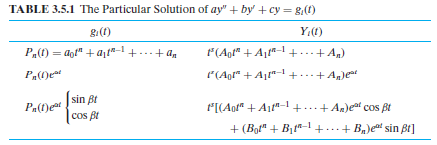
\includegraphics[width=345pt]{table.png}
    \end{center}
    